\documentclass{beamer}
\usepackage[utf8]{inputenc}
\usepackage[T1]{fontenc}

\usepackage{qtree}
\usepackage{dirtree}

\usebackgroundtemplate{
	
\includegraphics[width=\paperwidth,height=\paperheight]{img/background}
}

\title{Chapter 02: Other Classical Techniques}

\begin{document}
	\begin{frame}
		\titlepage
	\end{frame}

	\section{Introduction}
	\begin{frame}{Introduction}
		\begin{itemize}
		    \item Other classical techniques exists
		    \item We will review some of them, and later discuss about comparison
		    \item We will rarely use it, just so you know
		\end{itemize}
	\end{frame}
	
	\section{Finite State Machine}
	\begin{frame}{Finite State Machine}
    	\begin{itemize}
    	    \item Example originally from \cite{brady1977theory}: a safe has combination lock that can be in one out of three positions: 1, 2, and 3.
    	    \item It can go left (L) or right (R), hence 6 possible movements: 1L, 1R, 2L, 2R, 3L, 3R.
    	    \item Combination of the safe is 1L, 3R, 2L. Any other movement will set the alarm.
    	    \item Diagram here is made by free ``Qfsm'' tool.
	    \end{itemize}
	    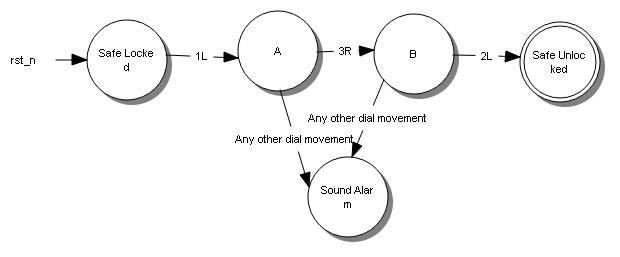
\includegraphics[scale=0.5]{img/03_safe_fsm.png}
	\end{frame}
	
	\section{References}
	\begin{frame}[allowframebreaks]
        \frametitle{References}
        \bibliographystyle{amsalpha}
        \bibliography{module_03}
	\end{frame}	
\end{document}
